\section{Overview and Reproducibility}
\label{app:overview}

This supplement gives the details behind each part of the main paper. It follows the same order as the paper: data and page types, statistics, the abstention test, page edits, the three fixes, the second domain, and ontology recovery. The last appendix covers two follow-up tests: a model that chooses the family on the page, and free-text answers. \Cref{tab:map} shows where each result of the main paper is explained in more depth. \Cref{fig:method} summarizes the four experiments in one picture.

\begin{figure}[t]
\centering
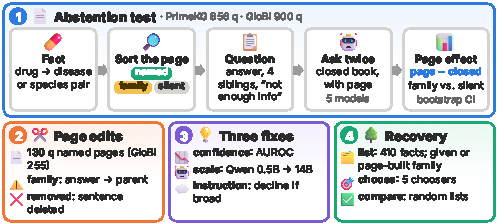
\includegraphics[width=\columnwidth]{figures/fig_method.pdf}
\caption{Our four experiments. (1) We sort each page as named, family-only or silent, and ask each question closed book and with the page. (2) We edit named pages: the answer becomes its family name, or we delete the sentence. (3) We test three fixes. (4) We try to recover the exact answer from the ontology.}
\label{fig:method}
\end{figure}

\begin{table}[t]
\centering
\footnotesize
\setlength{\tabcolsep}{3pt}
\begin{tabular}{@{}p{3.9cm}p{3.6cm}@{}}
\toprule
Main paper & Supplement \\
\midrule
Data, page types, \cref{M-tab:data,M-tab:coverage} & \cref{app:data} \\
Odds ratios, CIs, $p$-values, Eq.~\ref{M-eq:did} & \cref{app:stats} \\
Questions, prompts, \cref{M-tab:outcomes}, \cref{M-fig:forest} & \cref{app:questions} \\
Page edits, \cref{M-fig:edit} & \cref{app:edits} \\
Confidence, scale, instruction, \cref{M-fig:fixes} & \cref{app:fixes} \\
GloBI, \cref{M-tab:globi} & \cref{app:globi} \\
Recovery, \cref{M-tab:lists}, \cref{M-fig:recovery} & \cref{app:recovery} \\
Worked examples & \cref{app:cases} \\
Software and compute & \cref{app:compute} \\
Choosing the family, free text & \cref{app:followup} \\
\bottomrule
\end{tabular}
\caption{Where each part of the main paper is explained in this supplement.}
\label{tab:map}
\end{table}

\paragraph{Code and data.}
We release all code and derived data at \url{https://anonymous.4open.science/r/CLADE}. The release holds the question sets, the windowed pages, the candidate lists, the per-question model outputs, and every script that builds them. We do not redistribute Wikipedia or PubMed text; the scripts download it again from the public APIs. PrimeKG, MONDO, GloBI, Wikipedia and PubMed are all public.

\paragraph{Rerunning the numbers.}
Every table and figure comes from the shipped per-question outputs, so a reader can check them without a GPU or network access:
\begin{quote}
\footnotesize\ttfamily
bash tools/check\_results.sh\\
\# reruns the analysis and compares it\\
\# with results/; prints "identical: 22"
\end{quote}
The full pipeline, from raw downloads to the final tables, runs with one command on a SLURM cluster:
\begin{quote}
\footnotesize\ttfamily
bash run\_all.sh~~~~~~~~~~~~~\# PrimeKG\\
bash globi.sh all~~~~~~~~~~~~\# GloBI
\end{quote}
Both scripts resume where they stop, and a smoke test on small synthetic data checks the whole pipeline in a few minutes (\texttt{--smoke}).
